\documentclass[conference]{IEEEtran}
\usepackage{cite}
\usepackage{amsmath,amssymb,amsfonts}
\usepackage{algorithmic}
\usepackage{graphicx}
\usepackage{textcomp}
\usepackage{xcolor}
\usepackage{booktabs}
\usepackage{listings}
\usepackage{hyperref}

\def\BibTeX{{\rm B\kern-.05em{\sc i\kern-.025em b}\kern-.08em
    T\kern-.1667em\lower.7ex\hbox{E}\kern-.125emX}}

\begin{document}

\title{IntentGuard-eBPF: Dynamic, Microsecond-Level Runtime Containment for Autonomous LLM Agents}

\author{
\IEEEauthorblockN{Harikrishna D.}
}

\maketitle

\begin{abstract}
Autonomous Large Language Model (LLM) agents operating on local execution runtimes introduce critical attack surfaces, most notably indirect prompt injections that induce arbitrary subprocess spawning and remote data exfiltration. Existing container-level security frameworks (e.g., Tetragon, Falco) apply static seccomp/LSM policies at the container boundary, creating a semantic gap that ignores the granular, step-by-step reasoning lifecycle of AI agents. Conversely, MicroVM sandboxes (e.g., AWS Firecracker) enforce rigid isolation at severe resource and latency penalties. We present \textbf{IntentGuard-eBPF}, an open-source, zero-trust runtime containment system that bridges application-layer AI intent with kernel-space enforcement using Extended Berkeley Packet Filters (eBPF) and Compile Once -- Run Everywhere (CO-RE) primitives. IntentGuard exposes a microsecond-latency Userland-Kernel IPC socket bridge, allowing LLM SDKs to dynamically update eBPF Hash Maps immediately prior to high-risk tool execution. When an unauthorized syscall (\texttt{sys\_enter\_connect} or \texttt{sys\_enter\_execve}) is detected, the eBPF kernel program dispatches \texttt{SIGKILL} via \texttt{bpf\_send\_signal()}. Micro-benchmarks recorded an active-configuration \texttt{connect()} duration of $8.89\,\mu\text{s}$, an IPC round-trip mean of $31.66\,\mu\text{s}$, and a daemon resident memory mean of $14.24\,\text{MB}$. These measurements characterize the PoC on the evaluation host; they do not by themselves establish a causal comparison with virtualization.
\end{abstract}

\begin{IEEEkeywords}
eBPF, AI Agent Security, Runtime Security, Prompt Injection, Kernel Instrumentation, CO-RE, Zero-Trust Containment.
\end{IEEEkeywords}

\section{Introduction}
Autonomous agents powered by Large Language Models (LLMs) increasingly execute local system actions, including file retrieval, bash scripting, and API invocation. While extended agent capabilities enable automated workflows, they expose host systems to prompt injection vulnerabilities. In an indirect prompt injection attack, malicious instructions embedded within untrusted data inputs manipulate the agent into executing unauthorized operations, such as spawning interactive reverse shells or transmitting confidential system assets to external command-and-control (C2) servers.

Securing local agent execution presents a fundamental trade-off between performance and isolation context:
\begin{enumerate}
    \item \textbf{MicroVM and Container Isolation:} Solutions such as AWS Firecracker, E2B, and gVisor isolate execution environments within lightweight virtual machines or hypervisors. However, maintaining or dynamically provisioning microVM instances incurs multi-hundred millisecond cold-start latencies and substantial memory allocation ($>150\,\text{MB}$ per instance), rendering local multi-agent deployments resource-prohibitive.
    \item \textbf{Static Kernel-Level eBPF Security:} Tools like Cilium Tetragon and Sysdig Falco hook into Linux kernel tracepoints and LSM callbacks to detect suspicious system calls. However, these engines evaluate security rules against static pod or container boundaries. They operate blind to the agent's internal execution state, unable to differentiate between an agent legitimately requesting web access during a search tool phase versus executing unauthorized network requests during a local arithmetic evaluation step.
\end{enumerate}

To resolve this dichotomy, we introduce \textbf{IntentGuard-eBPF}, a lightweight framework that bridges the semantic gap between application-level agent reasoning and kernel-level syscall enforcement. By combining a Python context manager SDK, a Go control daemon utilizing \texttt{cilium/ebpf}, and a restricted C eBPF kernel module compiled via BPF CO-RE, IntentGuard enables dynamic, microsecond-granularity permission locking synchronized directly with agent reasoning loops.

\section{Threat Model \& Design Goals}

\subsection{Threat Model}
We assume an adversary who cannot directly modify the core agent code or host kernel, but can inject arbitrary text into the context window of an autonomous LLM agent (e.g., via web scraping, document parsing, or user input). The attacker's objective is to achieve arbitrary code execution on the underlying OS host by inducing the agent to execute two main attack primitives:
\begin{itemize}
    \item \textbf{Data Exfiltration Vector:} Initiating an outbound connection through \texttt{connect} to transmit environment variables, private files, or local keys to an untrusted external endpoint. The current PoC does not yet cover every network-send syscall.
    \item \textbf{Process Escalation Vector:} Executing a shell or other binary through \texttt{execve}. The current PoC does not yet hook \texttt{execveat} or automatically inherit policies across child processes.
\end{itemize}

\subsection{Design Goals}
\begin{enumerate}
    \item \textbf{Step-Aware Dynamic Enforcement:} Security policies must dynamically toggle permissions in real-time based on the specific tool or step active within the LLM reasoning chain.
    \item \textbf{Microsecond In-Kernel Intervention:} Unauthorized syscalls must be terminated instantly in kernel space via \texttt{SIGKILL} before network socket buffers (\texttt{sk\_buff}) or file handlers complete allocation.
    \item \textbf{Near-Zero Resource Footprint:} The system must run natively on host nodes with negligible memory usage ($<30\,\text{MB}$) and minimal latency impact ($<50\,\mu\text{s}$) per policy update.
\end{enumerate}

\section{System Architecture}

The IntentGuard-eBPF architecture consists of three decoupled operational tiers, as illustrated in Fig.~\ref{fig:arch}.

\begin{figure}[htbp]
\centering
\fbox{\parbox{0.9\linewidth}{\centering \textbf{[ Python LLM Agent SDK ]}\\ $\downarrow$ \textit{Unix Socket IPC (/tmp/intentguard.sock)}\\ \textbf{[ Go Userland Daemon (cilium/ebpf) ]}\\ $\downarrow$ \textit{eBPF BPF\_MAP\_TYPE\_HASH Updates}\\ \textbf{[ eBPF Kernel Hooks (sys\_enter\_connect / execve) ]}\\ $\downarrow$ \textit{Violation $\rightarrow$ bpf\_send\_signal(SIGKILL)}}}
\caption{Architectural overview of IntentGuard-eBPF showing the control pipeline from Python SDK down to eBPF kernel hooks.}
\label{fig:arch}
\end{figure}

\subsection{eBPF Kernel Program (Restricted C)}
The kernel layer attaches to two primary tracepoints: \texttt{syscalls/sys\_enter\_connect} and \texttt{syscalls/sys\_enter\_execve}. It maintains two BPF maps:
\begin{itemize}
    \item \texttt{policy\_map}: A \texttt{BPF\_MAP\_TYPE\_HASH} map indexed by task process ID (\texttt{u32 pid}). Values consist of a \texttt{policy\_t} struct containing single-byte flags \texttt{block\_network} and \texttt{block\_exec}.
    \item \texttt{events}: A \texttt{BPF\_MAP\_TYPE\_RINGBUF} ring buffer used to stream structured violation event logs (\texttt{event\_t}) to userland.
\end{itemize}

When a hook triggers, the kernel program extracts the active PID via \texttt{bpf\_get\_current\_pid\_tgid() >> 32} and queries \texttt{policy\_map}. If a matching record is present and the requested operation violates the policy flag (e.g., \texttt{block\_network == 1}), the program reserves an event slot in the ring buffer, records the process ID, violation type, and command name, submits the event, and invokes \texttt{bpf\_send\_signal(9)}. This dispatches an uncatchable \texttt{SIGKILL} from the kernel hook.

\subsection{Userland Control Daemon (Go)}
Developed in Go using \texttt{cilium/ebpf}, the daemon loads the compiled CO-RE ELF bytecode into kernel memory, attaches the tracepoints, and manages BPF map allocations. It exposes a low-latency Unix Domain Socket at \texttt{/tmp/intentguard.sock}. The daemon reads incoming JSON policy payloads from the socket and updates or deletes keys in \texttt{policy\_map} concurrently. Simultaneously, a dedicated Goroutine polls the BPF ring buffer reader to process security alerts.

\subsection{Developer SDK (Python)}
The Python SDK exposes an \texttt{IntentGuard} context manager that wraps arbitrary agent operations or tool callbacks (e.g., in LangChain or CrewAI). Upon entering the context block, the SDK determines the process ID (\texttt{os.getpid()}) and transmits a JSON payload to the Go daemon to lock permissions. Upon context exit, it issues a deletion payload to restore default process execution states.

\section{Implementation \& BPF CO-RE Verification}

IntentGuard-eBPF relies on BPF Compile Once -- Run Everywhere (CO-RE) to enable binary portability across heterogeneous kernel versions without requiring target-host LLVM toolchains or kernel source trees. Header types are generated directly via \texttt{bpftool btf dump file /sys/kernel/btf/vmlinux format c}.

The implementation satisfies the relevant Linux eBPF verifier constraints:
\begin{enumerate}
    \item Map lookups check for \texttt{NULL} pointers prior to dereferencing policy values.
    \item Ring buffer allocations check \texttt{bpf\_ringbuf\_reserve()} return pointers before writing event metadata.
    \item The generated object embeds BTF type information for the declared policy and event structures.
\end{enumerate}

\section{Experimental Evaluation}

We evaluated IntentGuard-eBPF on a bare-metal Linux host running kernel 6.8+ to quantify syscall hook overhead, IPC socket round-trip performance, and daemon resource consumption under heavy operational stress.

\subsection{Syscall Hook Overhead}
We executed 10,000 localhost TCP connection attempts while the daemon and eBPF tracepoint were active. The harness records end-to-end \texttt{connect()} call duration; it is not a controlled with/without-daemon differential measurement. As detailed in Table~\ref{tab:benchmarks}, the observed mean was $8.89\,\mu\text{s}$ ($0.00889\,\text{ms}$), with a median of $8.36\,\mu\text{s}$. The 99th percentile (P99) was $18.18\,\mu\text{s}$. These results establish a baseline for the active configuration, rather than isolating probe-only overhead.

\subsection{IPC Policy Update Round-Trip}
To evaluate dynamic policy switching, we executed 1,000 direct JSON request/ACK round trips between a Python benchmark client and the Go daemon over the Unix socket. The mean round-trip latency was $31.66\,\mu\text{s}$, with a median of $23.68\,\mu\text{s}$ and a P99 of $77.95\,\mu\text{s}$. This measures the control-plane socket path; SDK serialization and context-manager overhead are not separately isolated.

\subsection{Daemon Memory and CPU Footprint}
The Go daemon was profiled over 13,406 polling intervals while continuously handling approximately $1.34 \times 10^6$ dynamic policy updates. The daemon maintained a Resident Set Size (RSS) mean of $14.24\,\text{MB}$ ($14,236\,\text{KB}$), with a P99 of $15.28\,\text{MB}$ and a maximum of $16.42\,\text{MB}$. The benchmark records daemon CPU time as procfs tick counts; it does not convert those counts into host-independent utilization percentages.

\begin{figure}[htbp]
\centering
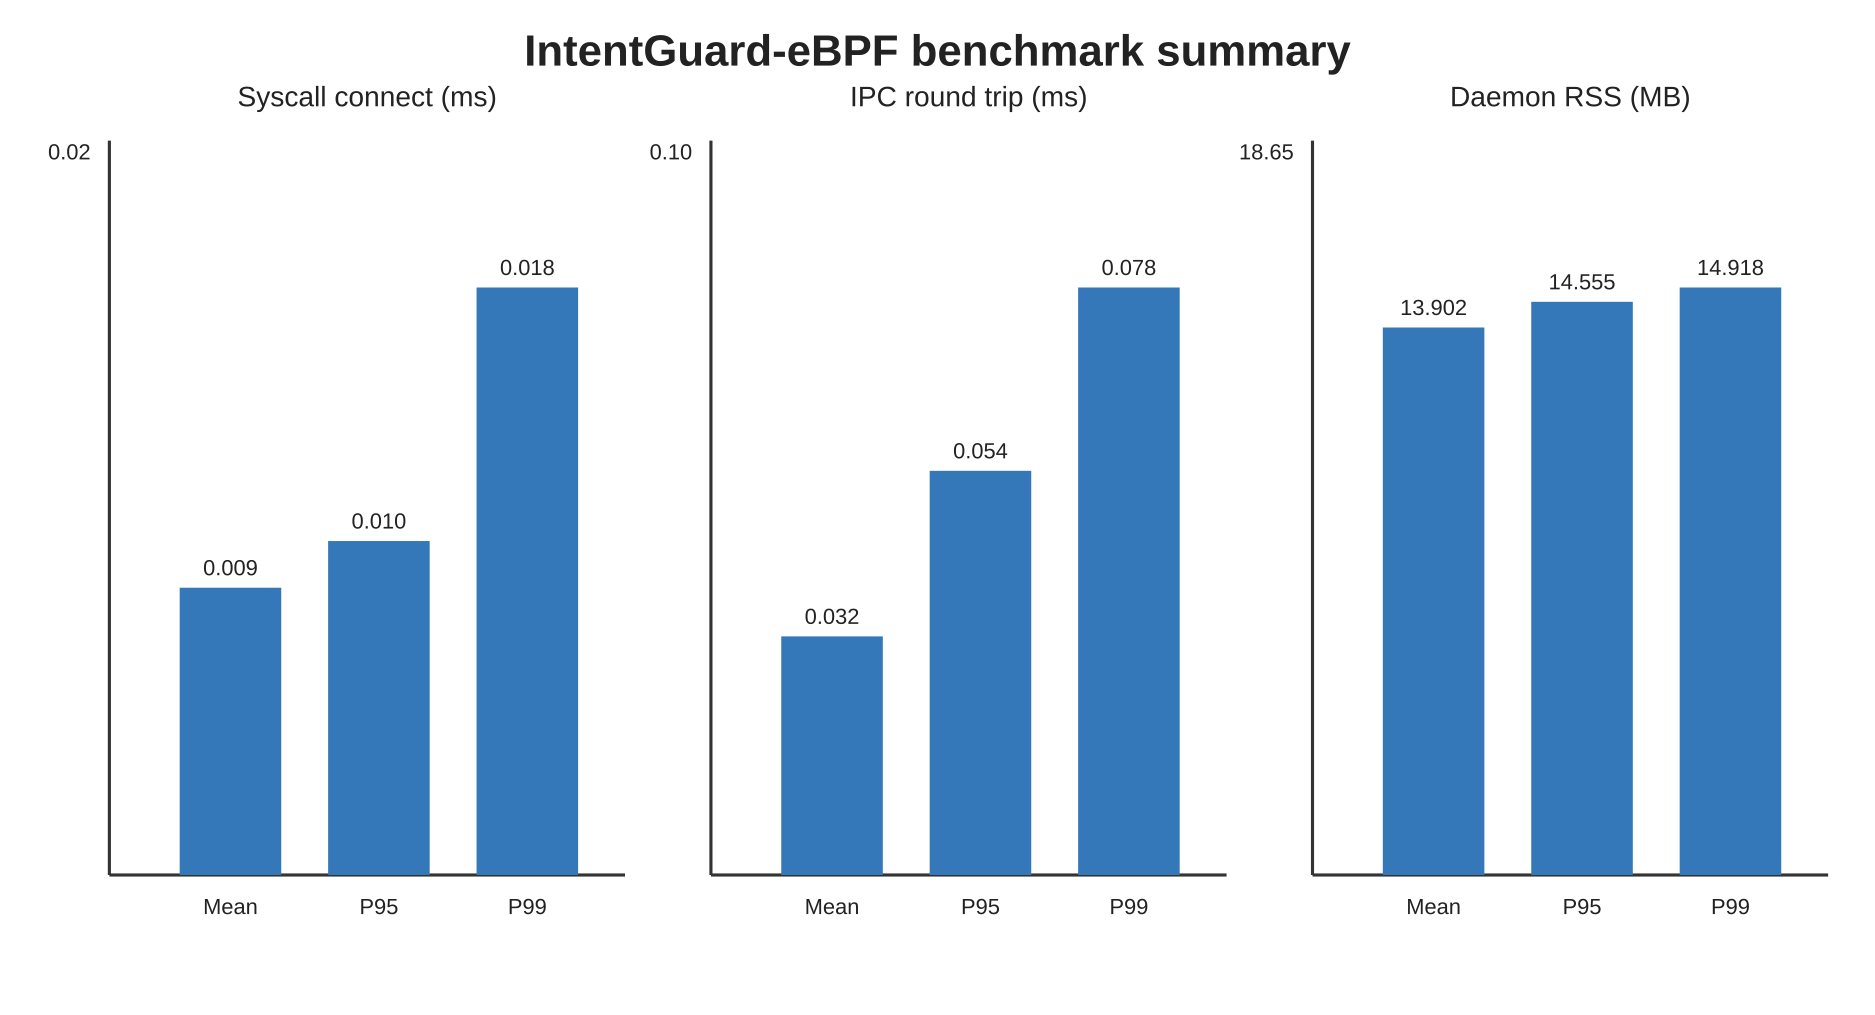
\includegraphics[width=\linewidth]{paper_benchmarks.png}
\caption{Mean, P95, and P99 values computed from the recorded syscall, IPC, and daemon RSS CSV samples. Syscall and IPC values are in milliseconds; RSS values are in megabytes.}
\label{fig:benchmarks}
\end{figure}

\begin{table}[htbp]
\caption{Empirical Benchmark Performance Metrics}
\label{tab:benchmarks}
\centering
\begin{tabular}{lrrrr}
\toprule
\textbf{Metric} & \textbf{Mean} & \textbf{Median} & \textbf{P95} & \textbf{P99} \\
\midrule
Syscall Latency ($\mu\text{s}$) & 8.89 & 8.36 & 10.34 & 18.18 \\
IPC Round-Trip ($\mu\text{s}$) & 31.66 & 23.68 & 53.63 & 77.95 \\
Daemon Memory (MB) & 14.24 & 14.14 & 14.90 & 15.28 \\
\bottomrule
\end{tabular}
\end{table}

\subsection{Comparative Analysis}
Table~\ref{tab:comparison} contrasts IntentGuard-eBPF against state-of-the-art isolation paradigms across key architectural dimensions.

\begin{table}[htbp]
\caption{Comparative Security \& Architectural Summary}
\label{tab:comparison}
\centering
\begin{tabular}{p{2.2cm}p{1.6cm}p{1.8cm}p{1.8cm}}
\toprule
\textbf{Architecture} & \textbf{Startup Latency} & \textbf{RAM Footprint} & \textbf{Step Context} \\
\midrule
MicroVMs (Firecracker) & Reported externally & Reported externally & Static VM boundary \\
Generic eBPF (Tetragon) & Reported externally & Reported externally & Static Pod boundary \\
\textbf{IntentGuard-eBPF} & \textbf{31.66\,$\mu\text{s} mean IPC} & \textbf{14.24\,MB mean RSS} & \textbf{PID-scoped policy} \\
\bottomrule
\end{tabular}
\end{table}

\section{Conclusion \& Future Work}
IntentGuard-eBPF addresses the semantic gap in autonomous AI agent containment by coupling application-level intent with kernel-level eBPF enforcement. By leveraging BPF CO-RE and a low-latency IPC daemon, IntentGuard dynamically locks down network access and subprocess execution for the current process, with an observed active-configuration \texttt{connect()} duration of $8.89\,\mu\text{s}$ and a daemon RSS mean of $14.24\,\text{MB}$. Controlled baseline comparisons, broader syscall coverage, and child-process policy inheritance remain important future work.

Future work includes extending eBPF tracepoint hooks to LSM security modules (\texttt{bpf\_lsm}) for fine-grained file path matching, as well as developing native plugins for major agentic frameworks including LangGraph, CrewAI, and AutoGen.

\section*{Acknowledgment}

\begin{thebibliography}{00}
\bibitem{bpf2go} Cilium eBPF Library for Go, \url{https://github.com/cilium/ebpf}, 2026.
\bibitem{tetragon} Isovalent Tetragon: eBPF-based Security Observability and Enforcement, \url{https://github.com/cilium/tetragon}, 2026.
\bibitem{firecracker} A. Agache et al., ``Firecracker: Lightweight Virtualization for Serverless Applications,'' in \textit{Proc. USENIX NSDI}, 2020.
\bibitem{ebpf_core} A. Nakryiko, ``BPF CO-RE (Compile Once -- Run Everywhere),'' Linux Kernel Documentation, 2021.
\end{thebibliography}

\end{document}